\documentclass{standalone}
\usepackage{tikz}

\begin{document}
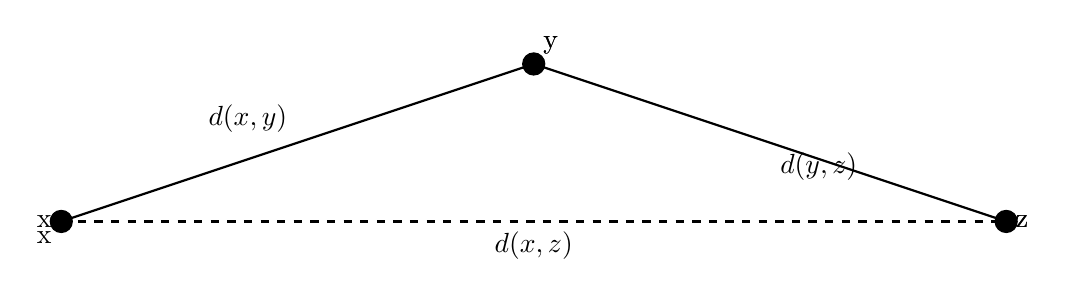
\begin{tikzpicture}[scale=2]
    % Define points
    \coordinate (x) at (-3,0);
    \coordinate (y) at (0,1);
    \coordinate (z) at (3,0);

    % Draw points
    \filldraw[black] (x) circle (2pt) node[left] {x};
    \filldraw[black] (y) circle (2pt) node[above right] {y};
    \filldraw[black] (z) circle (2pt) node[right] {z};

    % Draw paths
    \draw[->,thick] (x) -- (y) node[midway, above left] {$d(x,y)$};
    \draw[->,thick] (y) -- (z) node[midway, below right] {$d(y,z)$};
    \draw[->,thick,dashed] (x) -- (z) node[midway, below] {$d(x,z)$};

    % Labeling
    \node[below left] at (x) {x};
    \node[above right] at (y) {y};
    \node[right] at (z) {z};
\end{tikzpicture}
\end{document}